\documentclass{standalone}
\usepackage{amsmath, amsfonts}
\usepackage{pgfplots}
\pgfplotsset{compat=1.16}

\begin{document}

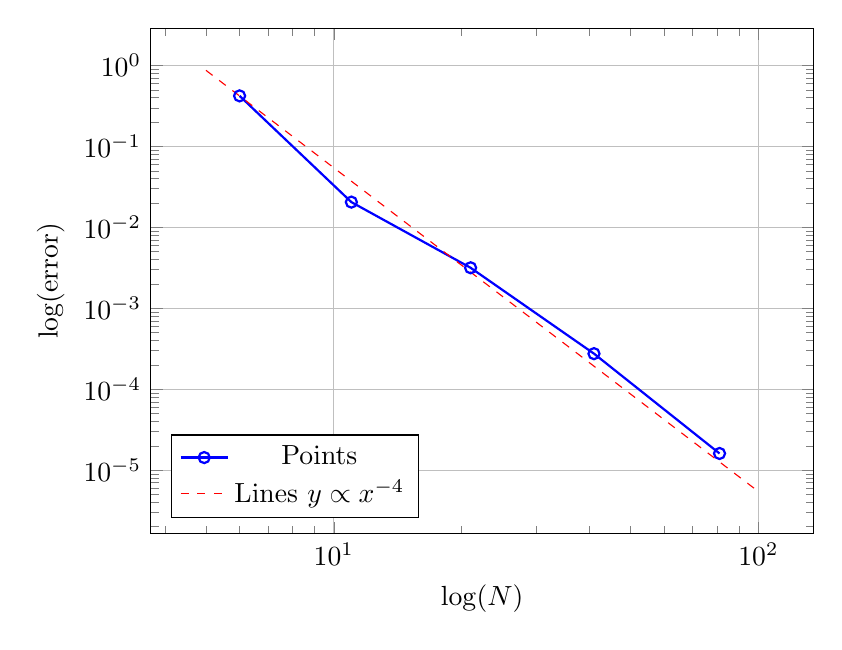
\begin{tikzpicture}
\begin{loglogaxis}[
    width=10cm,
    height=8cm,
    xlabel={$\log(N)$},
    ylabel={$\log(\text{error})$},
    grid=major,
    legend pos=south west
]
\addplot[
    mark=o,
    color=blue,
    thick
] coordinates {
    (6, 0.421705)
    (11, 0.0205289)
    (21, 0.00316894)
    (41, 0.000275356)
    (81, 1.609e-5)
};
\addlegendentry{Points}

\addplot[
    mark=none,
    color=red,
    dashed,
    domain=5:100
] {544.78*x^-4};
\addlegendentry{Lines $y \propto x^{-4}$}
\end{loglogaxis}
\end{tikzpicture}

\end{document}
